\documentclass[a4paper,14pt]{extarticle}

\usepackage[utf8x]{inputenc}
\usepackage[T1]{fontenc}
\usepackage[russian]{babel}
\usepackage{hyperref}
\usepackage{indentfirst}
\usepackage{here}
\usepackage{array}
\usepackage{graphicx}
\usepackage{grffile}
\usepackage{caption}
\usepackage{subcaption}
\usepackage{chngcntr}
\usepackage{amsmath}
\usepackage{amssymb}
\usepackage{pgfplots}
\usepackage{pgfplotstable}
\usepackage[left=2cm,right=2cm,top=2cm,bottom=2cm,bindingoffset=0cm]{geometry}
\usepackage{multicol}
\usepackage{multirow}
\usepackage{titlesec}
\usepackage{listings}
\usepackage{color}
\usepackage{longtable}
\usepackage{enumitem}
\usepackage{cmap}
\usepackage{tikz}

\usetikzlibrary{shapes,arrows}

\definecolor{green}{rgb}{0,0.6,0}
\definecolor{gray}{rgb}{0.5,0.5,0.5}
\definecolor{purple}{rgb}{0.58,0,0.82}

\lstset{
	language={C},
	inputpath={logs},
	backgroundcolor=\color{white},
	commentstyle=\color{green},
	keywordstyle=\color{blue},
	numberstyle=\scriptsize\color{gray},
	stringstyle=\color{purple},
	basicstyle=\small,
	breakatwhitespace=false,
	breaklines=true,
	captionpos=b,
	keepspaces=true,
	numbers=left,
	numbersep=5pt,
	showspaces=false,
	showstringspaces=false,
	showtabs=false,
	tabsize=8,
	frame=single,
}

\renewcommand{\le}{\ensuremath{\leqslant}}
\renewcommand{\leq}{\ensuremath{\leqslant}}
\renewcommand{\ge}{\ensuremath{\geqslant}}
\renewcommand{\geq}{\ensuremath{\geqslant}}
\renewcommand{\epsilon}{\ensuremath{\varepsilon}}
\renewcommand{\phi}{\ensuremath{\varphi}}
\renewcommand{\thefigure}{\arabic{figure}}
\def\code#1{\texttt{#1}}

\titleformat*{\section}{\large\bfseries} 
\titleformat*{\subsection}{\normalsize\bfseries} 
\titleformat*{\subsubsection}{\normalsize\bfseries} 
\titleformat*{\paragraph}{\normalsize\bfseries} 
\titleformat*{\subparagraph}{\normalsize\bfseries} 

\counterwithin{figure}{section}
\counterwithin{equation}{section}
\counterwithin{table}{section}
\newcommand{\sign}[1][5cm]{\makebox[#1]{\hrulefill}}
\newcommand{\equipollence}{\quad\Leftrightarrow\quad}
\newcommand{\no}[1]{\overline{#1}}
\graphicspath{{figs/}}
\captionsetup{justification=centering,margin=1cm}
\def\arraystretch{1.3}
\setlength\parindent{5ex}
\titlelabel{\thetitle.\quad}

\setitemize{itemsep=0em}
\setenumerate{itemsep=0em}

\tikzstyle{startstop} = [
	rectangle,
	align=center,
	rounded corners,
	text width=10em,
	text centered,
	draw=black
]
\tikzstyle{process} = [
	rectangle,
	align=center,
	text width=20em,
	text centered,
	draw=black
]
\tikzstyle{decision} = [
	diamond,
	aspect=4,
	align=center,
	inner sep=0pt,
	text width=10em,
	text centered,
	node distance=5em,
	draw=black
]
\tikzstyle{line} = [
	draw=black,
	thick,
	->,
	>=stealth,
	-latex'
]

\begin{document}

\begin{titlepage}
\begin{center}
	САНКТ-ПЕТЕРБУРГСКИЙ ПОЛИТЕХНИЧЕСКИЙ УНИВЕРСИТЕТ\\ ПЕТРА ВЕЛИКОГО\\[0.3cm]
	\par\noindent\rule{10cm}{0.4pt}\\[0.3cm]
	Институт компьютерных наук и технологий \\[0.3cm]
	Кафедра компьютерных систем и программных технологий\\[4cm]
	
	Реферат\\[3mm]
	Дисциплина: <<Защита информации>>\\[3mm]
	Тема: <<Обзор основных нововведений в Федеральном законе\\ от 27.07.2006 N 149-ФЗ (ред. от 19.07.2018)\\ <<Об информации, информационных технологиях и о защите информации>>\\[7cm]
\end{center}

\begin{flushleft}
	\hspace*{5mm} Выполнил студент гр. 43501/3  \hspace*{1.5cm}\sign[3cm]\hfill А.Ю. Ламтев\\
	\hspace*{9.4cm} (подпись)\\[3mm]
	\hspace*{5mm} Преподаватель \hspace*{5.0cm}\sign[3cm]\hfill А.Г. Новопашенный\\
	\hspace*{9.4cm} (подпись)\\[5mm]
	\hspace*{11.1cm} <<\sign[7mm]>> \sign[27mm] \the\year\hspace{1mm} г.
\end{flushleft}

\vfill

\begin{center}
	Санкт-Петербург\\
	\the\year
\end{center}
\end{titlepage}
\addtocounter{page}{1}

\tableofcontents
\listoffigures
\listoftables
\newpage

\section{Цель работы}

Научиться анализировать сетевой трафик при помощи программы \code{WireShark}.

\section{Программа работы}

Проанализировать сетевой трафик:

\begin{enumerate}
	\item Протокола ARP
	\item Протокола ICMP
	\begin{itemize}
		\item ping без фрагментации
		\item ping с фрагментацией
		\item tracert
		\item ошибки 3/1
	\end{itemize}
	\item Протокола UDP
	\item Протокола TCP
\end{enumerate}

\section{Условия сети}

Часть работы была выполнена в сети кафедры. Её конфигурация представлена в листинге \ref{lst:net-kspt}.

\lstinputlisting[caption={Конфигурация сети кафедры},label={lst:net-kspt},basicstyle=\scriptsize]{ifconfig-kspt.txt}


Другая часть работы была выполнена в домашней сети, конфигурация которой представлена в листинге \ref{lst:net-home}.

\lstinputlisting[caption={Конфигурация домашней сети},label={lst:net-home},basicstyle=\scriptsize]{ifconfig-home.txt}

\section{Протокол ARP}

Рассмотрим принцип действия протокола ARP. Выполним широковещательный ARP-запрос, отправив ping пакет другому узлу сети по адресу \code{10.1.99.131}.  На рис. \ref{fig:arp-req} представлен ARP-пакет.

\begin{figure}[H]
	\centering
	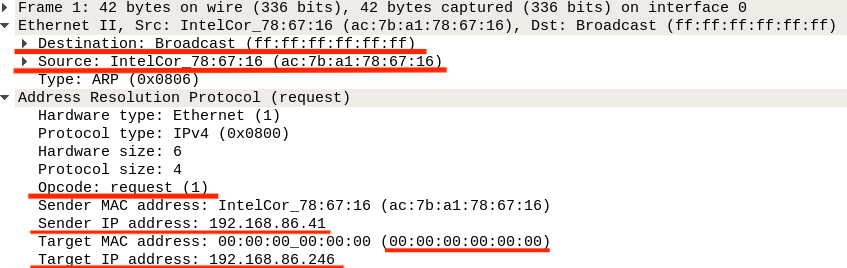
\includegraphics[width=1\textwidth]{arp-req}
	\caption{ARP-запрос}
	\label{fig:arp-req}
\end{figure}

Затем, узел сети по адресу \code{10.1.99.131} отправляет широковещательный ARP-ответ, который представлен на рис. \ref{fig:arp-resp}

\begin{figure}[H]
	\centering
	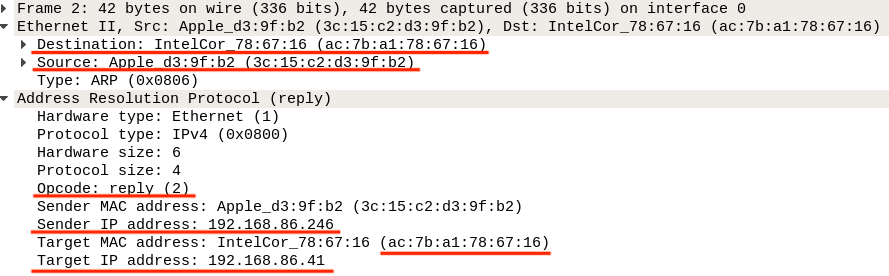
\includegraphics[width=1\textwidth]{arp-resp}
	\caption{ARP-ответ}
	\label{fig:arp-resp}
\end{figure}

После этого он отправляет широковещательный ARP-запрос с целью узнать наш ip адрес. И наконец, мы отправляем ARP-ответ. Эти 2 ARP-пакета представлены на рис. \ref{fig:arp-req2} и \ref{fig:arp-resp2} соответственно. 

\begin{figure}[H]
	\centering
	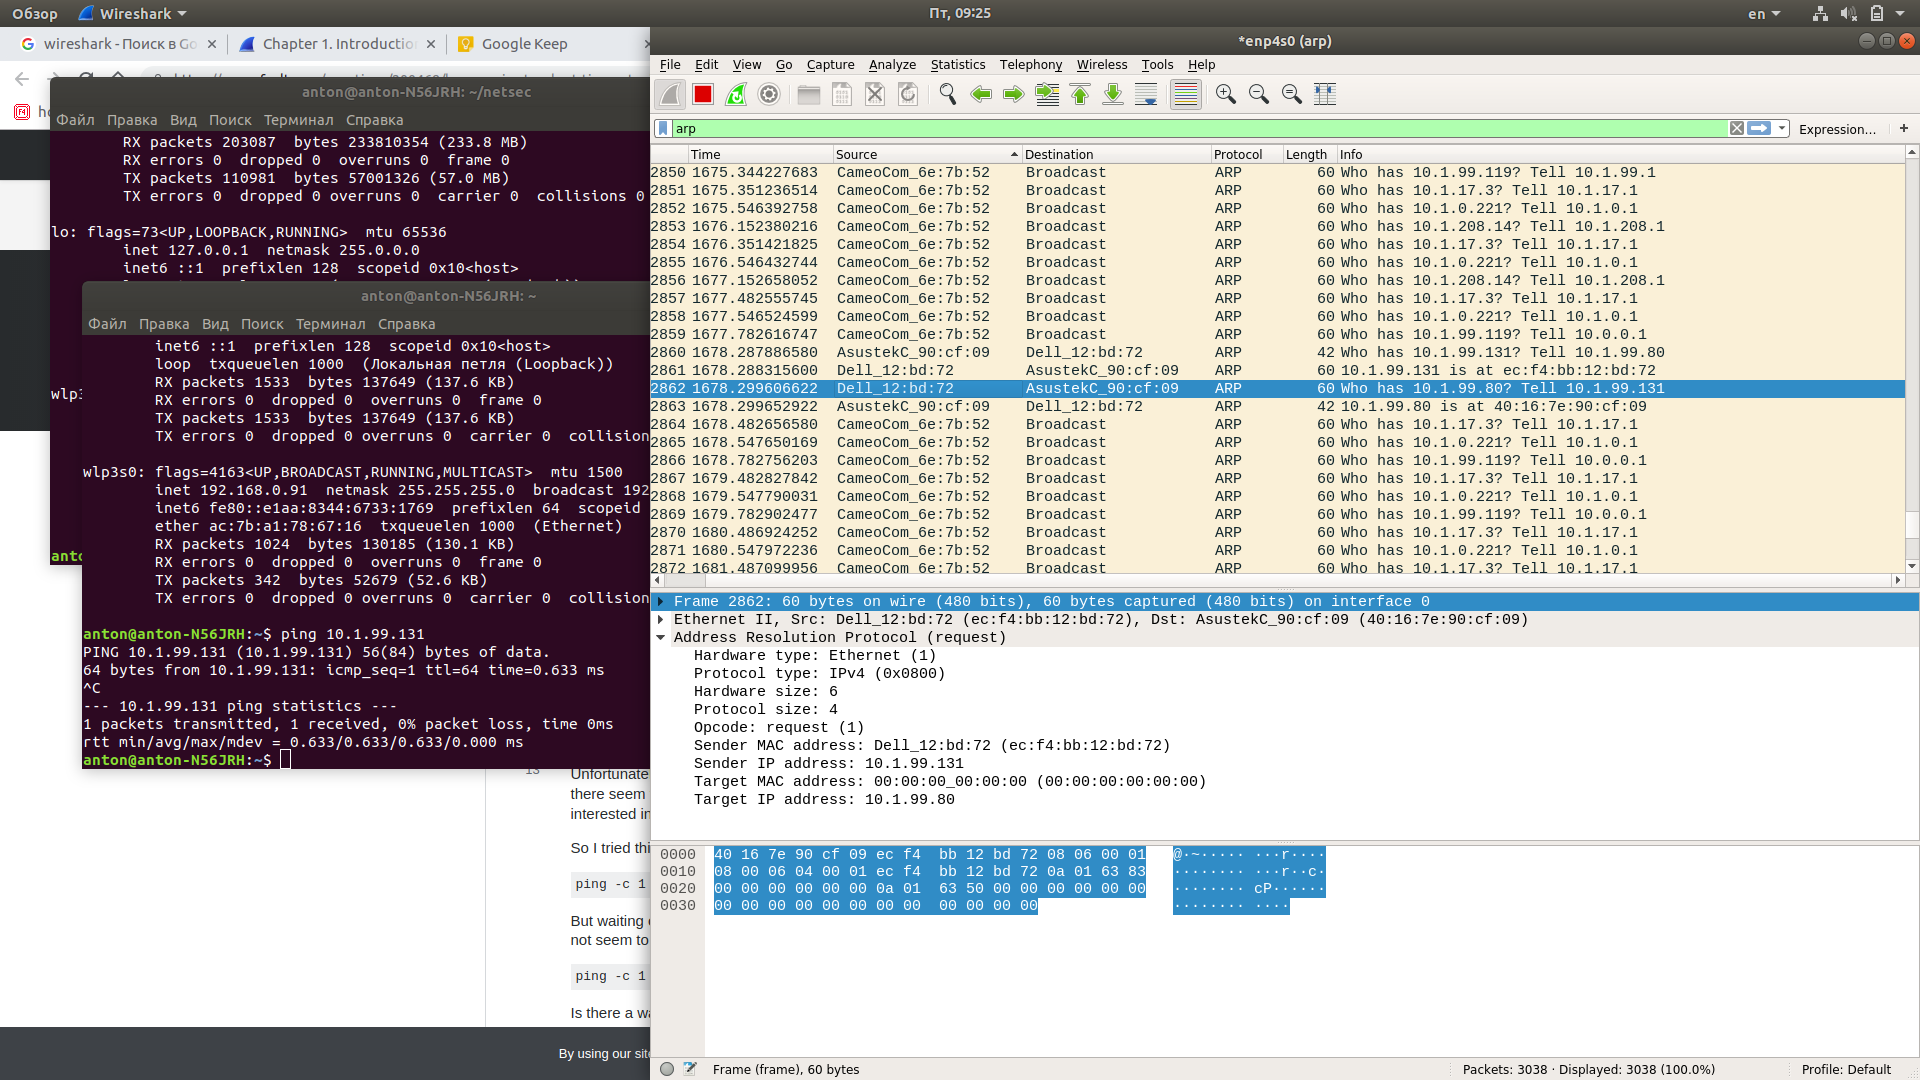
\includegraphics[width=1\textwidth]{arp-req2}
	\caption{ARP-запрос}
	\label{fig:arp-req2}
\end{figure}

\begin{figure}[H]
	\centering
	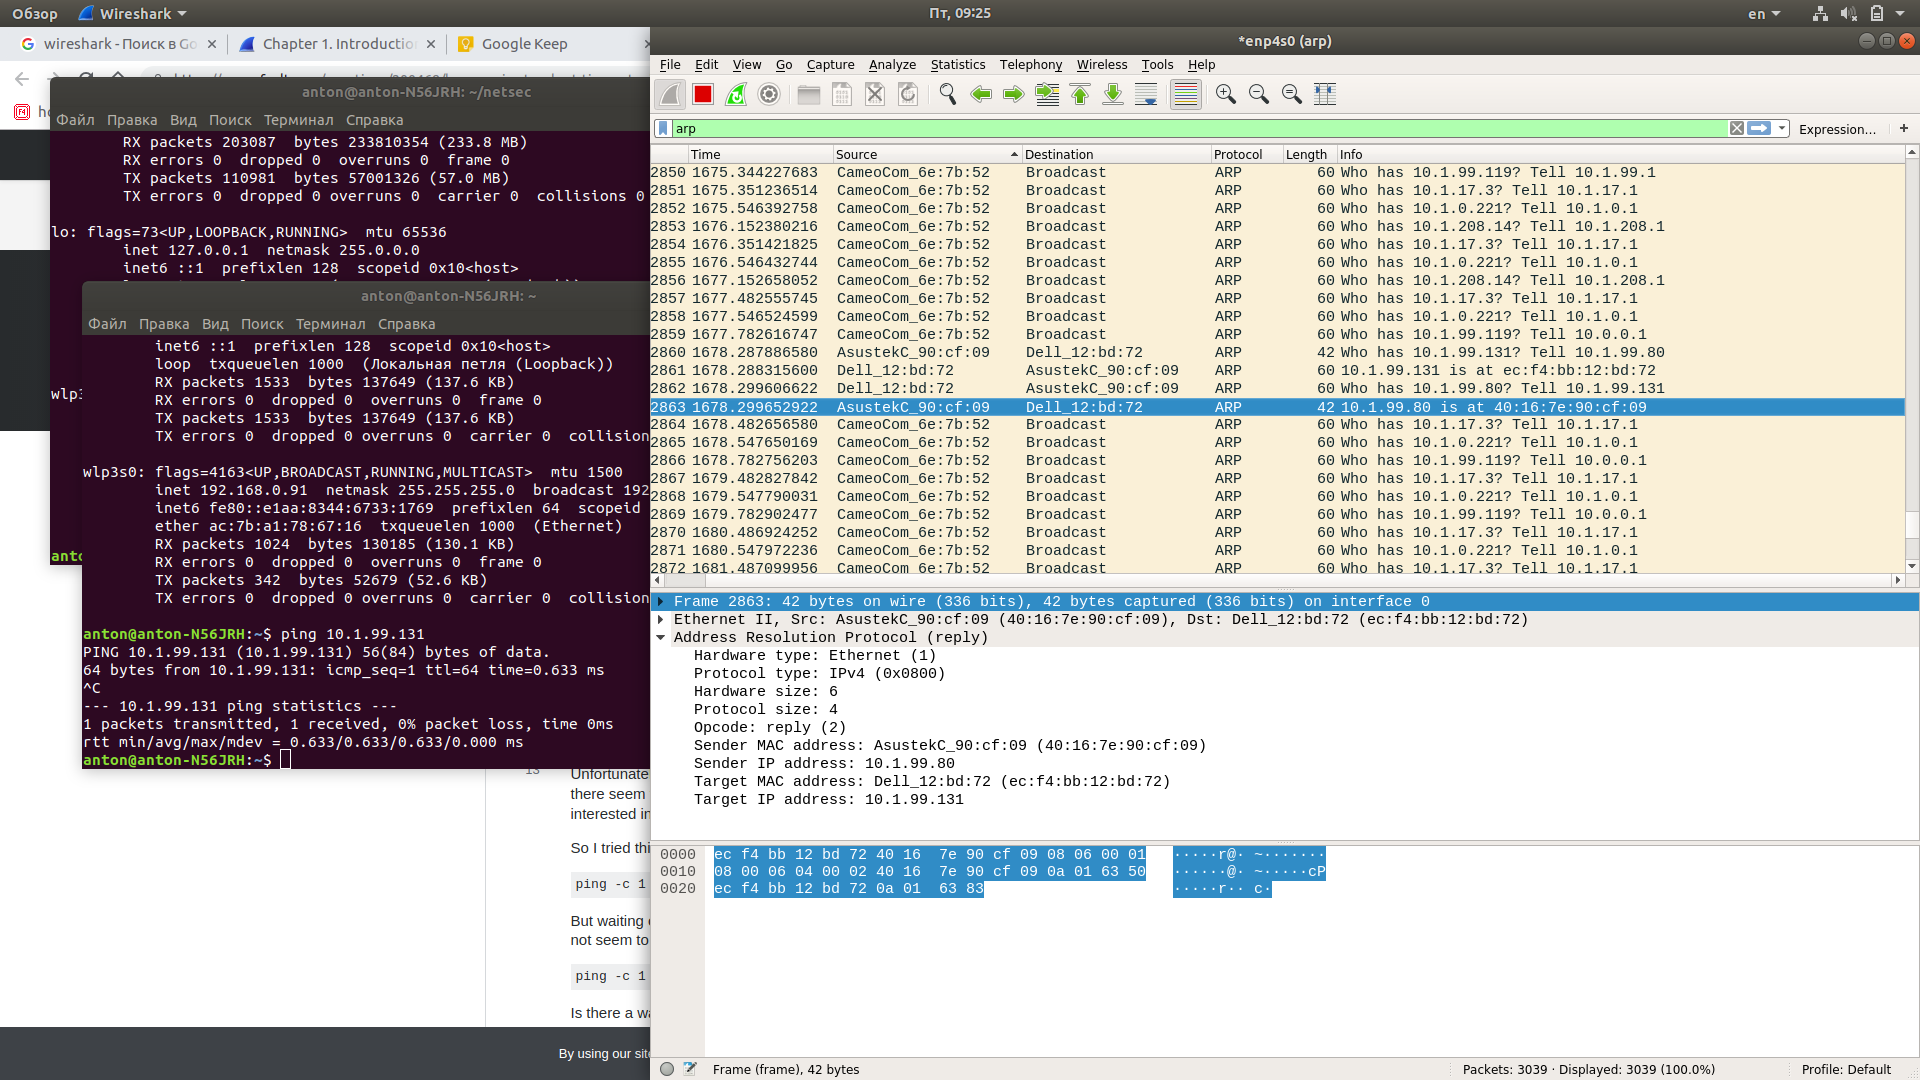
\includegraphics[width=1\textwidth]{arp-resp2}
	\caption{ARP-ответ}
	\label{fig:arp-resp2}
\end{figure}

\section{Протокол ICMP}

\subsection{Утилита ping}

Утилита ping отправляет ICMP эхо-запрос, на который, в случае успеха приходит ICMP эхо-ответ. Если пакет не пришел за определённое время, то удалённый хост считается недостижимым.

\paragraph{Ping без фрагментации}

\paragraph{Ping с фрагментацией}



\section{Протокол UDP}

\section{Протокол TCP}

\section{Выводы}

\end{document}
